\subsubsection*{u.1 Registrazione di un nuovo utente}

Dopo aver determinato il volume dei dati ed aver associato a ciascuna operazione principale richiesta la frequenza di esecuzione procediamo ad esaminare gli schemi di navigazione per le principali operazioni richieste.
\begin{longtblr}
[
  caption = {Registrazione di un nuovo utente},
]{
  colspec = {|X[3]X[1]X[2]X[4]|},
  rowhead = 1,
  hlines,
  row{even} = {lightgray},
  row{1} = {LightCoral},
} 
Concetto & Costrutto & Accessi & Tipo\\
Users & E & 1 & Scrittura \\
\SetCell[c=4]{l, white} {
  Totale: 1S \textrightarrow 300/giorno\\
  Costo totale: 300 x (1) = 300/giorno
  }

\end{longtblr}


\subsubsection*{u2. Login di un utente}
\begin{longtblr}
[
  caption = {Login di un utente},
]{
  colspec = {|X[3]X[1]X[2]X[4]|},
  rowhead = 1,
  hlines,
  row{even} = {lightgray},
  row{1} = {LightCoral},
} 
Concetto & Costrutto & Accessi & Tipo\\
Users & E & 1 & L\\ 
\SetCell[c=4]{l, white} {
  Totale: 1L \textrightarrow 1500/giorno\\
  Costo totale: 300 x (1) = 1500/giorno
  }

\end{longtblr}

\subsubsection*{u3. Modificare i dati del proprio account}
\begin{longtblr}
  [
    caption = {Modificare i dati del proprio account},
  ]{
    colspec = {|X[3]X[1]X[2]X[4]|},
    rowhead = 1,
    hlines,
    row{even} = {lightgray},
    row{1} = {LightCoral},
  } 
  Concetto & Costrutto & Accessi & Tipo\\
  Users & E & 1 & L\\ 
  \SetCell[c=4]{l, white} {
  Totale: 1S \textrightarrow 300/giorno\\
  Costo totale: 300 x (1) = 300/giorno
  }
  \end{longtblr}


%%%%%% ADMIN %%%%%%%
\subsubsection*{a1. Consultare la lista degli enti}
Per ogni ente recupero l'utente che lo ha creato e la media delle recensioni.\\
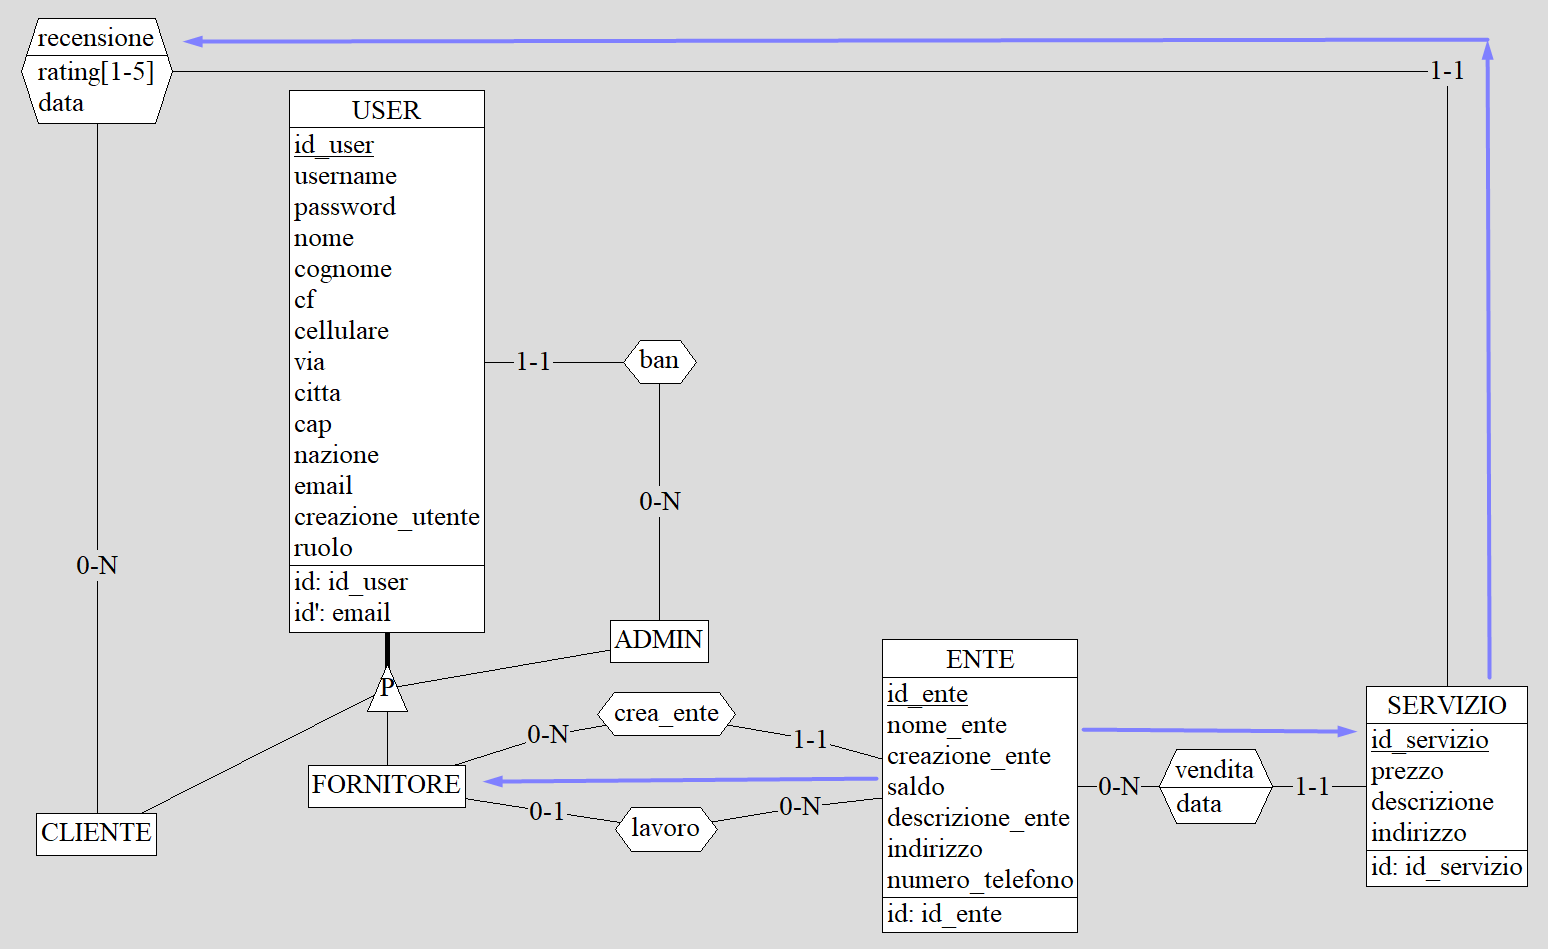
\includegraphics[width=0.95\columnwidth]{a1getUser.png}
\begin{longtblr}
  [
    caption = {Consultare la lista degli enti},
  ]{
    colspec = {|X[3]X[1]X[2]X[4]|},
    rowhead = 1,
    hlines,
    row{even} = {lightgray},
    row{1} = {LightCoral},
  } 
  Concetto & Costrutto & Accessi & Tipo\\
  Ente & E & 1 & L\\ 
  \SetCell[c=4]{l, white} {
    Totale: 1L \textrightarrow 50/giorno\\
    Costo totale: 50 x (1) = 50/giorno
    }

  \end{longtblr}


  \subsubsection*{a2. Bannare gli altri utenti}
  \begin{longtblr}
    [
      caption = {Bannare gli altri utenti},
    ]{
      colspec = {|X[3]X[1]X[2]X[4]|},
      rowhead = 1,
      hlines,
      row{even} = {lightgray},
      row{1} = {LightCoral},
    } 
    Concetto & Costrutto & Accessi & Tipo\\
    Users & E & 1 & L\\
    Ban & R & 1 & L \\ 
    \SetCell[c=4]{c} {Totale: 1S \textrightarrow 5/giorno}
    \SetCell[c=4]{l, white} {
      Totale: 2L\textrightarrow 5/giorno\\
      Costo totale: 5 x (2) = 10/giorno
      }
  \end{longtblr}


%%% TODO 
\subsubsection*{a3. Reset delle recensioni}
\begin{longtblr}
[
caption = {Reset delle recensioni},
]{
colspec = {|X[3]X[1]X[2]X[4]|},
rowhead = 1,
hlines,
row{even} = {lightgray},
row{1} = {LightCoral},
} 
Concetto & Costrutto & Accessi & Tipo\\
Ente & E & 1 & L \\
Vendita & R & 1 & L \\
Servizio & E & 1 & L\\ 
Recensione & R & 1 & L \\
Recensione & R & 1 & S \\

\SetCell[c=4]{l, white} {
    Totale: 4L + 1S \textrightarrow 1/giorno\\
    Costo totale: 1 x (5) = 5/giorno
    }
\end{longtblr}


Verranno eseguite le query necessarie per ottenere le seguenti statistiche:\\
\begin{itemize}
  \item numero check-in
  \item numero check-in falliti
  \item numero CityCard attive
  \item numero eventi attivi
  \item numero servizi attivi
\end{itemize}

\subsubsection*{a4. Consultare le statistiche}
\begin{longtblr}
[
caption = {Consultare statistiche},
]{
colspec = {|X[3]X[1]X[2]X[4]|},
rowhead = 1,
hlines,
row{even} = {lightgray},
row{1} = {LightCoral},
} 
Concetto & Costrutto & Accessi & Tipo\\
Users & E & 1 & L\\ 
\SetCell[c=4]{l, white} {
    Totale: 1L \textrightarrow 5/giorno\\
    Costo totale: 1 x (5) = 5/giorno
    }
\end{longtblr}


\subsubsection*{f1. Creare enti}
\begin{longtblr}
[
caption = {Creare enti},
]{
colspec = {|X[3]X[1]X[2]X[4]|},
rowhead = 1,
hlines,
row{even} = {lightgray},
row{1} = {LightCoral},
} 
Fornitore & E & 1 & L\\ 
Crea Ente & R & 1 & S \\
Ente & E & 1 & L \\
\SetCell[c=4]{l, white} {
    Totale: 2L + 1S \textrightarrow 8/giorno\\
    Costo totale: 3 x (8) = 15/giorno
    }
\end{longtblr}


\subsubsection*{f2. Associarsi a un ente}
\begin{longtblr}
[
caption = {Associarsi a un ente},
]{
colspec = {|X[3]X[1]X[2]X[4]|},
rowhead = 1,
hlines,
row{even} = {lightgray},
row{1} = {LightCoral},
} 
Concetto & Costrutto & Accessi & Tipo\\
Fornitore & E & 1 & L\\ 
Lavora & R & 1 & S \\ 
Ente & E & 1 & L \\
\SetCell[c=4]{l, white} {
    Totale: 2L + 1S \textrightarrow 3/giorno\\
    Costo totale: 3 x (3) = 9/giorno
    }
\end{longtblr}

\subsubsection*{f3. Creare servizi}
\begin{longtblr}
[
caption = {Creare servizi},
]{
colspec = {|X[3]X[1]X[2]X[4]|},
rowhead = 1,
hlines,
row{even} = {lightgray},
row{1} = {LightCoral},
} 
Concetto & Costrutto & Accessi & Tipo\\
Ente & E & 1 & L\\ 
Vende & R & 1 & S \\
Servizio & E & 1 & L \\
\SetCell[c=4]{l, white} {
    Totale: 2L + 1S\textrightarrow 10/giorno\\
    Costo totale: 3 x (10) = 30/giorno
    }
\end{longtblr}


\subsubsection*{f4. Creare eventi occasionali}
\begin{longtblr}
[
caption = {Creare eventi occasionali},
]{
colspec = {|X[3]X[1]X[2]X[4]|},
rowhead = 1,
hlines,
row{even} = {lightgray},
row{1} = {LightCoral},
} 
Concetto & Costrutto & Accessi & Tipo\\
Ente & E & 1 & L\\ 
Organizza & R & 1 & S \\
Occasionale & E & 1 & L \\
\SetCell[c=4]{l, white} {
    Totale: 2L + 1S \textrightarrow 4/giorno\\
    Costo totale: 3 x (4) = 12/giorno
    }
\end{longtblr}



Per creare un evento periodico si dovrà ottenere l'id dell'ente al quale è associato il fornitore, poi andare a creare un record per l'evento e un altro record per il periodo. \\
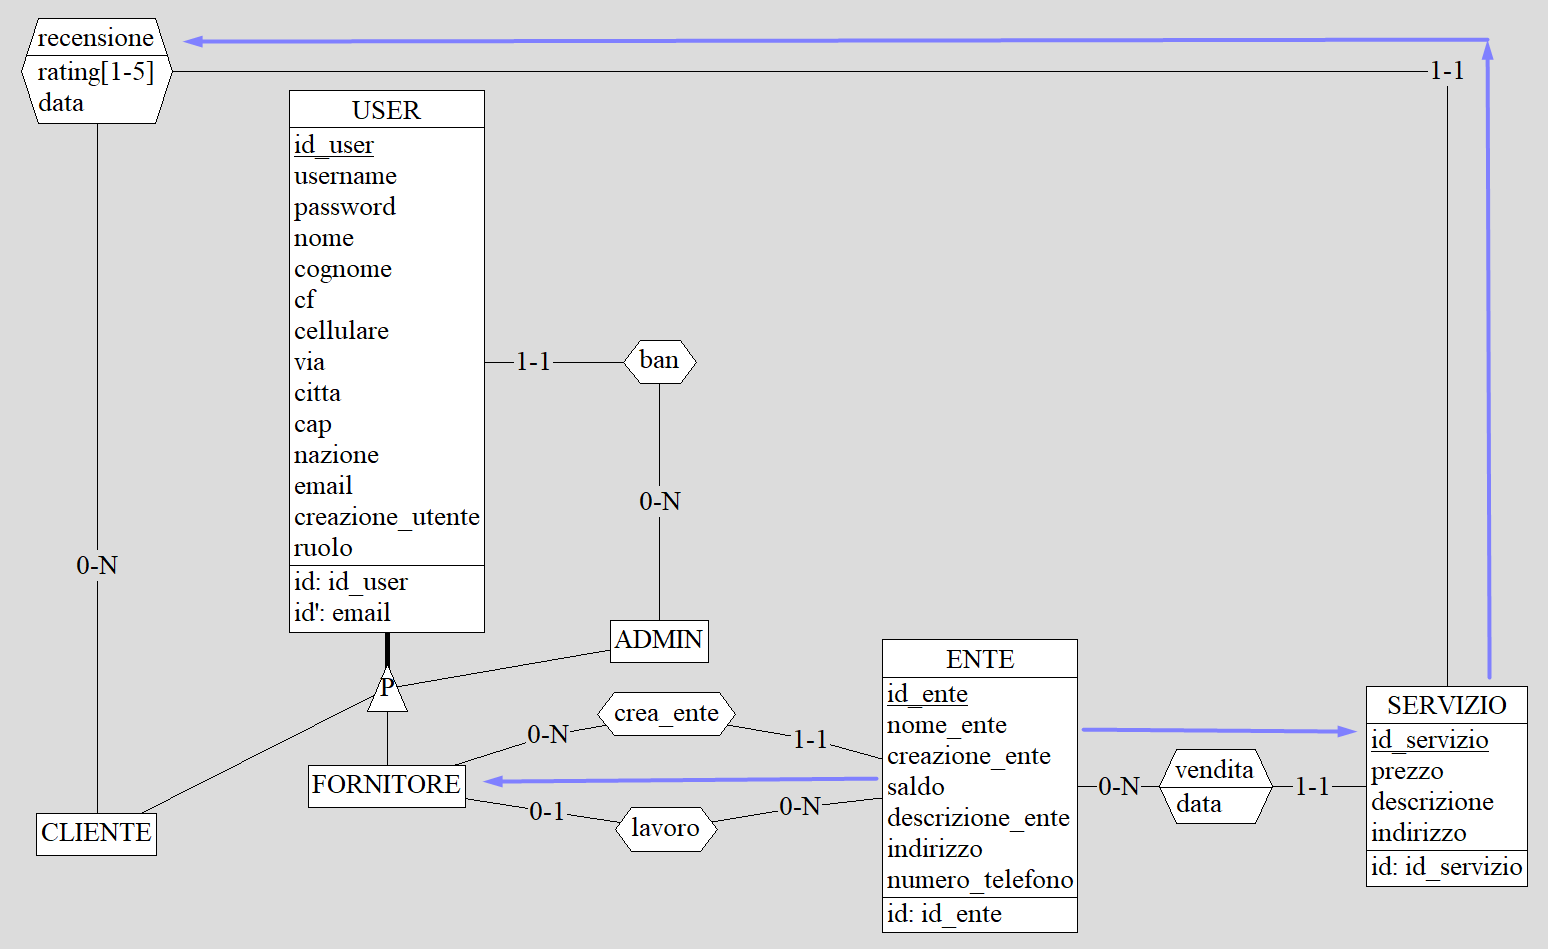
\includegraphics[width=0.95\columnwidth]{a1getUser.png}

\subsubsection*{f5. Creare eventi periodici}
\begin{longtblr}
[
caption = {Creare eventi periodici},
]{
colspec = {|X[3]X[1]X[2]X[4]|},
rowhead = 1,
hlines,
row{even} = {lightgray},
row{1} = {LightCoral},
} 
Concetto & Costrutto & Accessi & Tipo\\
Ente & E & 1 & L\\ 
Organizza & R & 1 & S \\
Periodico & E & 1 & L \\
\SetCell[c=4]{l, white} {
    Totale: 2L + 1S \textrightarrow 1/giorno\\
    Costo totale: 3 x (1) = 4/giorno
    }
\end{longtblr}



Oltre alla query per ottenere il'id dell'ente del fornitore verranno eseguite quelle necessarie per ottenere le seguenti statistiche:\\
\begin{itemize}
  \item saldo dell'ente associato al fornitore
  \item numero eventi attivi
  \item numero servizi attivi
\end{itemize}

\subsubsection*{f6. Consultare statistiche riguardo il proprio ente}
\begin{longtblr}
[
caption = {Consultare statistiche riguardo il proprio ente},
]{
colspec = {|X[3]X[1]X[2]X[4]|},
rowhead = 1,
hlines,
row{even} = {lightgray},
row{1} = {LightCoral},
} 
Concetto & Costrutto & Accessi & Tipo\\
Fornitore & E & 1 & L\\ 
Ente & E & 1 & L \\
\SetCell[c=4]{l, white} {
    Totale: 2L \textrightarrow 800/giorno\\
    Costo totale: 2 x (800) = 1600/giorno
    }
\end{longtblr}


\subsubsection*{c1. Richiedere una CityCard}
\begin{longtblr}
[
caption = {Richiedere una CityCard},
]{
colspec = {|X[3]X[1]X[2]X[4]|},
rowhead = 1,
hlines,
row{even} = {lightgray},
row{1} = {LightCoral},
} 
Concetto & Costrutto & Accessi & Tipo \\
Cliente & E & 1 & L\\ 
Possesso CityCard & R & 1 & S \\
CityCard & E & 1 & L \\
\SetCell[c=4]{l, white} {
    Totale: 2L + 1S \textrightarrow 2000/giorno\\
    Costo totale: 5 x (2000) = 6000/giorno
    }
\end{longtblr}

Prima di sottoscrivere un abbonamento vengono cercate una CityCard valida e una carta di credito predefinita. \\
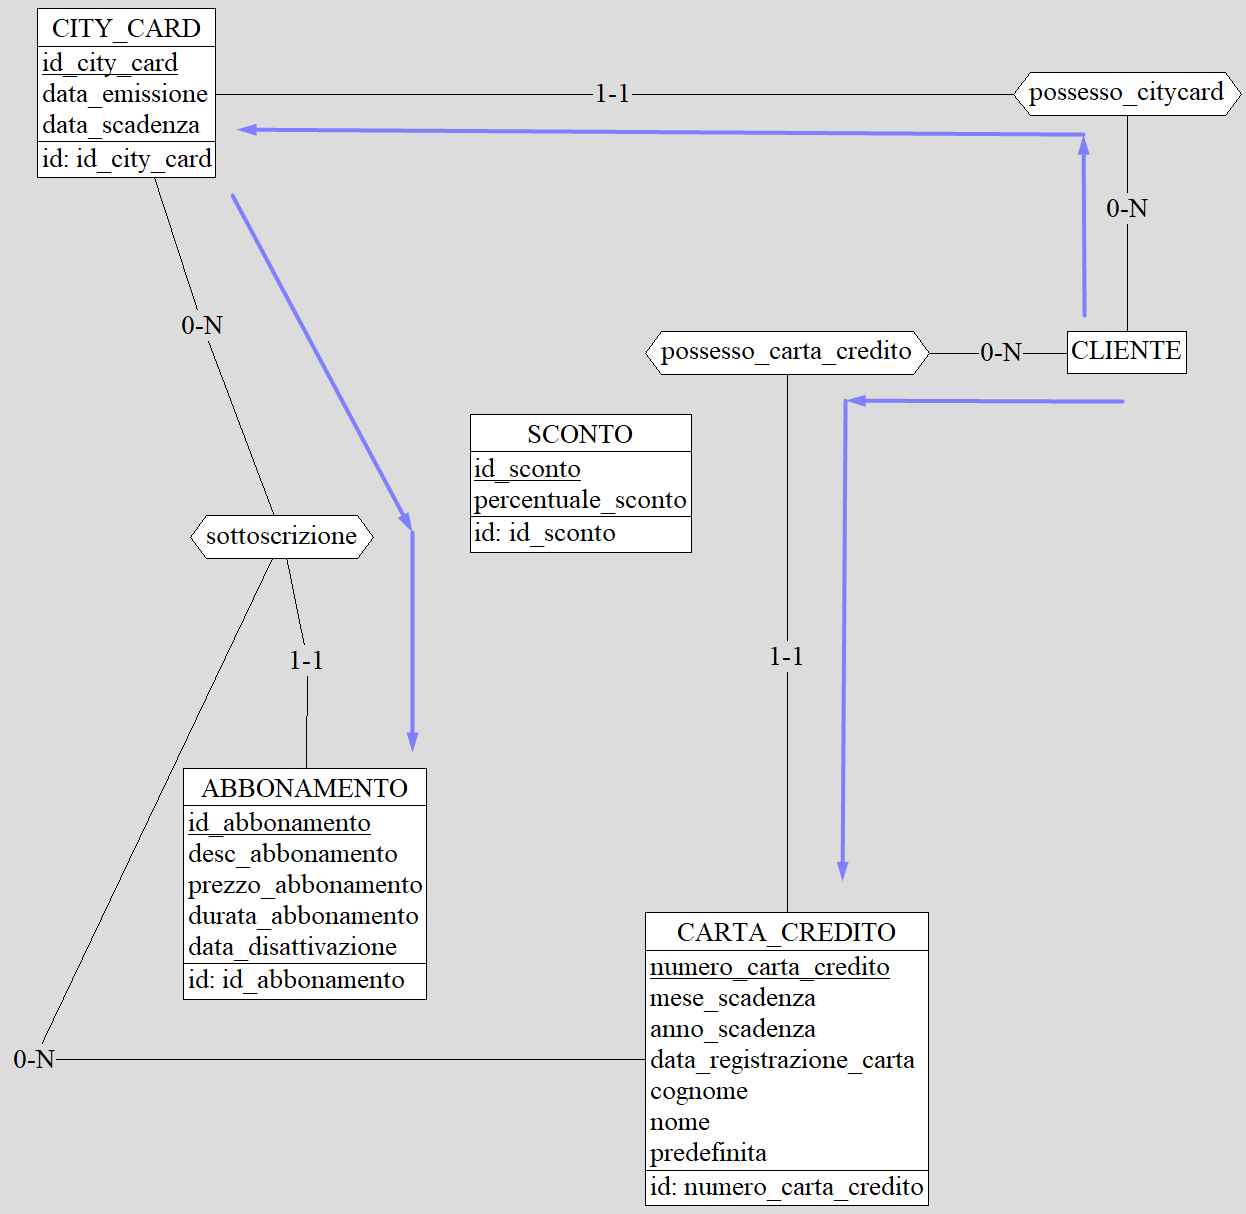
\includegraphics[width=0.95\columnwidth]{c2sottoscrizioneAbbonamento.png}

\subsubsection*{c2. Sottoscrivere un abbonamento}
\begin{longtblr}
[
caption = {Sottoscrivere un abbonamento},
]{
colspec = {|X[3]X[1]X[2]X[4]|},
rowhead = 1,
hlines,
row{even} = {lightgray},
row{1} = {LightCoral},
} 
Concetto & Costrutto & Accessi & Tipo \\
Cliente & E & 1 & L\\ 
Possesso Carta di credito & R & 1 & L \\
Carta Credito & E & 1 & L \\
Sottoscrizione & R & 1 & S \\
Abbonamento & E & 1 & L \\
\SetCell[c=4]{l, white} {
    Totale: 2L + 1S \textrightarrow 2000/giorno\\
    Costo totale: 3 x (2000) = 6000/giorno
    }
\end{longtblr}


\subsubsection*{c3. Aggiungere una carta di credito}
\begin{longtblr}
[
caption = {Aggiungere una carta di credito},
]{
colspec = {|X[3]X[1]X[2]X[4]|},
rowhead = 1,
hlines,
row{even} = {lightgray},
row{1} = {LightCoral},
} 
Concetto & Costrutto & Accessi & Tipo \\
Cliente & E & 1 & L\\ 
Carta credito & R & S \\
\SetCell[c=4]{l, white} {
    Totale: 1L + 1S \textrightarrow 2000/giorno\\
    Costo totale: 2 x (2000) = 4000/giorno
    }
\end{longtblr}


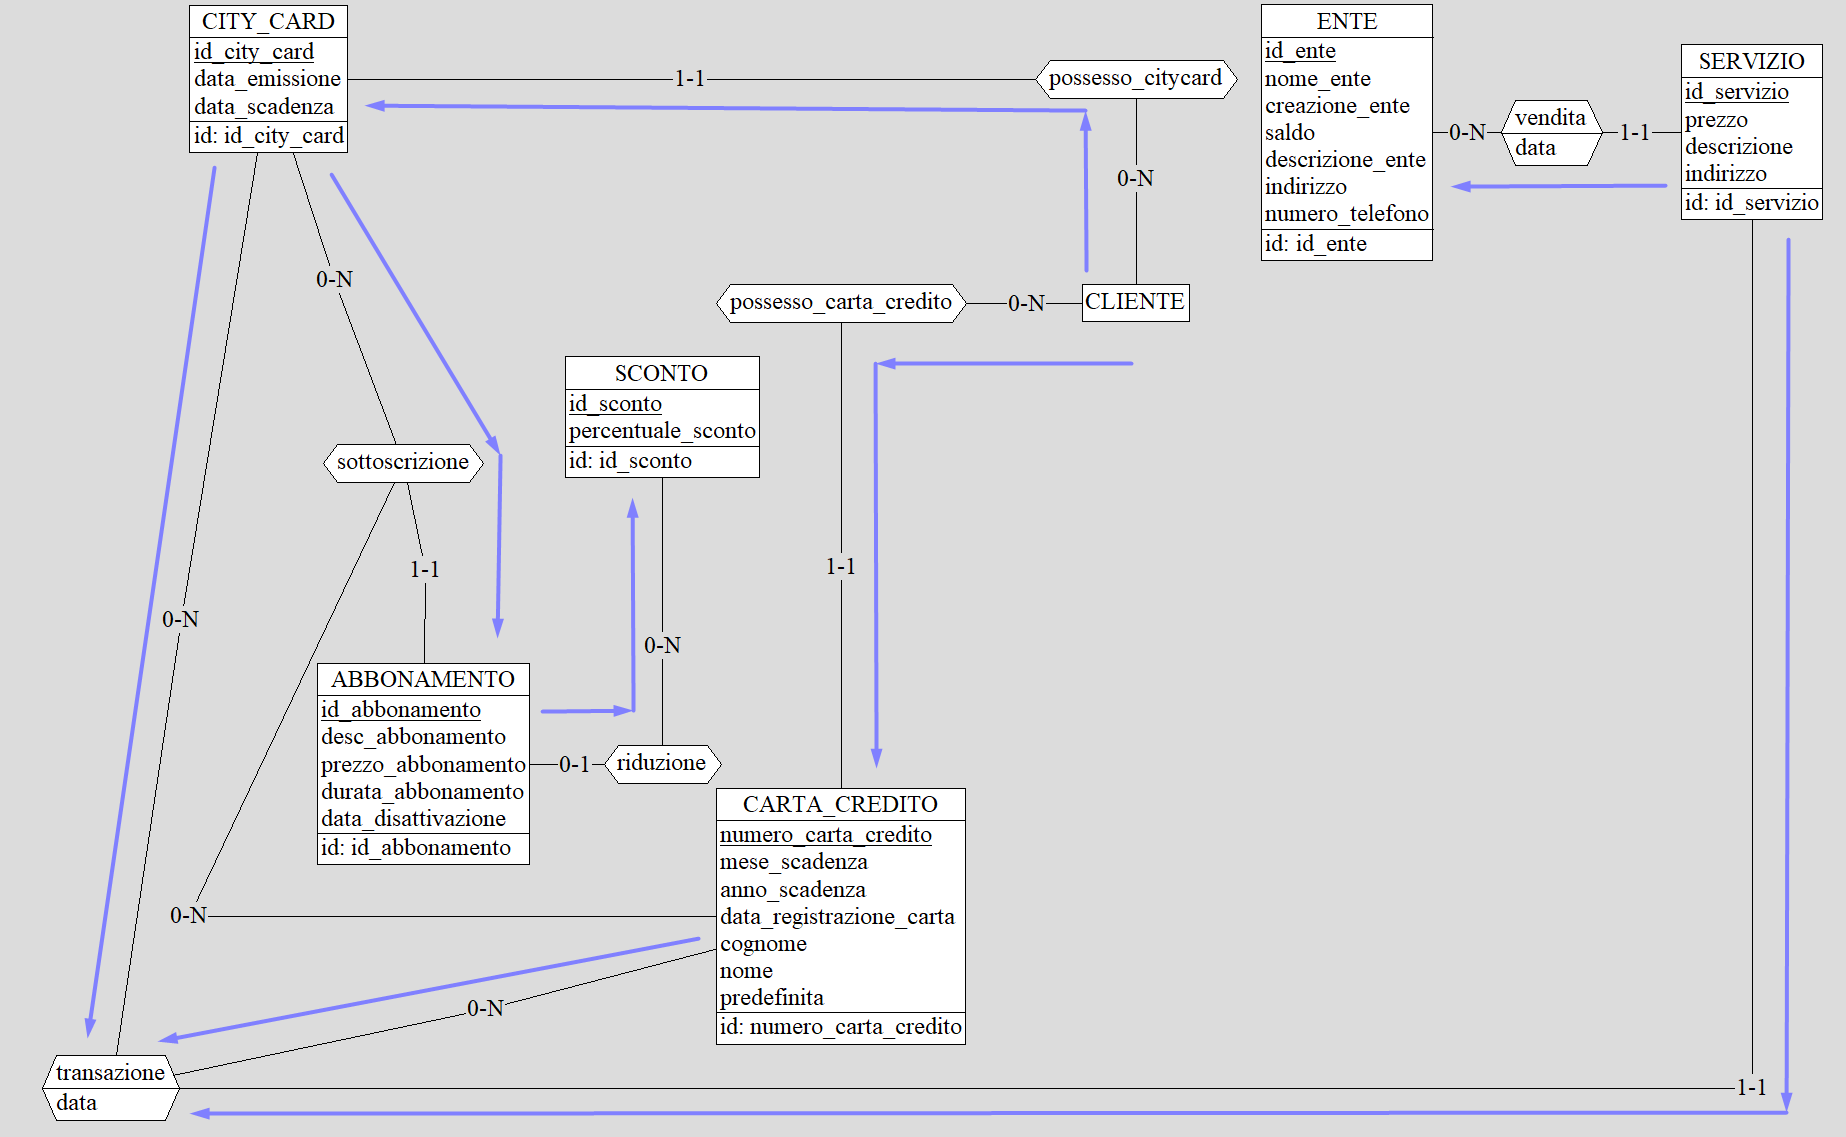
\includegraphics[width=0.95\columnwidth]{c5acquistaServizio.png}

\subsubsection*{c4. Acquistare un servizio}
\begin{longtblr}
[
caption = {Acquistare un servizio},
]{
colspec = {|X[3]X[1]X[2]X[4]|},
rowhead = 1,
hlines,
row{even} = {lightgray},
row{1} = {LightCoral},
} 
Concetto & Costrutto & Accessi & Tipo \\
Enti & E & 1 & L\\ 
Servizi & E & 1 & L\\ 
Carta di credito & E & 1 & L\\ 
CityCard & E & 1 & L\\ 
Sconti & E & 1 & L\\ 
Abbonamenti & E & 1 & L\\ 
Sottoscrizione & E & 1 & L\\ 
Servizi & E & 1 & L\\ 
Transazione & E & 1 & R\\ 
\SetCell[c=4]{l, white} {
    Totale: 8L + 1S \textrightarrow 3000/giorno\\
    Costo totale: 9 x (3000) = 27000/giorno
    }
\end{longtblr}

\subsubsection*{c5. Prenotare un evento}
\begin{longtblr}
[
caption = {Prenotare un evento},
]{
colspec = {|X[3]X[1]X[2]X[4]|},
rowhead = 1,
hlines,
row{even} = {lightgray},
row{1} = {LightCoral},
} 
Concetto & Costrutto & Accessi & Tipo \\
Cliente & E & 1 & L \\
Partecipazione & R & 1 & S \\
Eventi & E & 1 & L\\ 
\SetCell[c=4]{l, white} {
    Totale: 2L + 1S \textrightarrow 500/giorno\\
    Costo totale: 3 x (500) = 1500/giorno
    }
\end{longtblr}


Per poter effettuare un check-in devo confermare che la CityCard del cliente sia valida.
\subsubsection*{c6. Effettuare un check-in}
\begin{longtblr}
[
caption = {Effettuare un check-in},
]{
colspec = {|X[3]X[1]X[2]X[4]|},
rowhead = 1,
hlines,
row{even} = {lightgray},
row{1} = {LightCoral},
} 
Concetto & Costrutto & Accessi & Tipo \\
CityCard & E & 1 & L\\ 
Checkin completato & R & 1 & S\\
Trasporto pubblico & E & 1 & L \\
Checkin fallito & R & 1 & S \\
Errore & E & 1 & L \\   % TODO verificare
\SetCell[c=4]{l, white} {
    Totale: 3L + 2S \textrightarrow 5000/giorno\\
    Costo totale: 5 x (5000) = 25000/giorno
    }
\end{longtblr}

\subsubsection*{c7. Consultare la lista degli acquisti fatti}
\begin{longtblr}
[
caption = {Consultare la lista degli acquisti fatti},
]{
colspec = {|X[3]X[1]X[2]X[4]|},
rowhead = 1,
hlines,
row{even} = {lightgray},
row{1} = {LightCoral},
} 
Concetto & Costrutto & Accessi & Tipo \\
servizi acquistati & E & 1 & L\\ 
Cliente & E & 1 & L\\ 
Servizi & E & 1 & L\\ 
\SetCell[c=4]{l, white} {
    Totale: 2L \textrightarrow 3000/giorno\\
    Costo totale: 2 x (3000) = 6000/giorno
    }
\end{longtblr}


%% TODO  calcolare ridondanze
\subsubsection*{c8. Lasciare una recensione riguardo un servizio acquistato}
\begin{longtblr}
[
caption = {Lasciare una recensione riguardo un servizio acquistato},
]{
colspec = {|X[3]X[1]X[2]X[4]|},
rowhead = 1,
hlines,
row{even} = {lightgray},
row{1} = {LightCoral},
} 
Concetto & Costrutto & Accessi & Tipo \\
servizi acquistati & E & 1 & L\\ 
Cliente & E & 1 & L\\ 
Recensione & R & 1 & S \\
Servizio & E & 1 & L \\

\SetCell[c=4]{l, white} {
    Totale: 2L + 1S \textrightarrow 1500/giorno\\
    Costo totale: 3 x (1500) = 4500/giorno
    }
\end{longtblr}



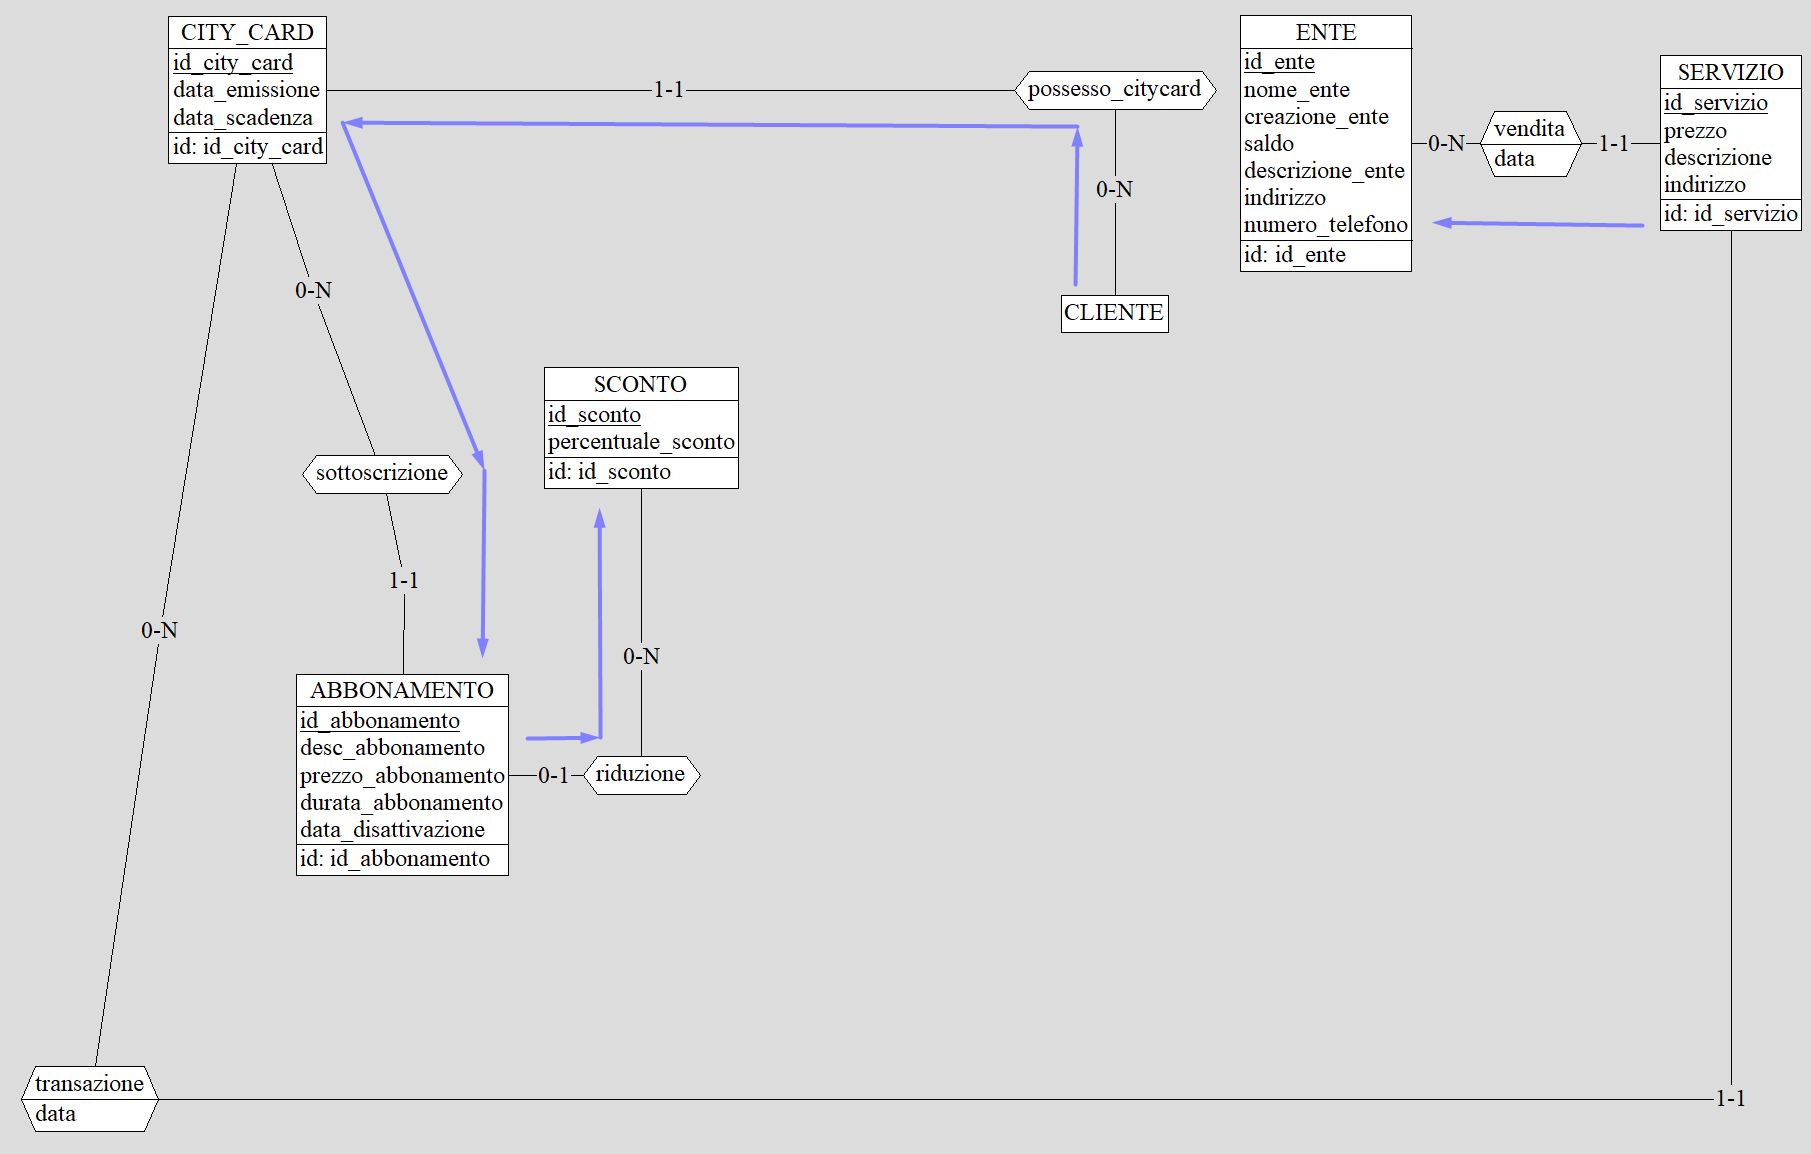
\includegraphics[width=0.95\columnwidth]{c10getServizi.png}
\\
\\
Nella tabella dei servizi disponibili si dovrà mettere anche l'ente fornitore, il prezzo scontato in base all'abbonamento sottoscritto dal cliente.
\subsubsection*{c9. Visualizzare lista servizi}
\begin{longtblr}
[
caption = {Visualizzare lista servizi},
]{
colspec = {|X[3]X[1]X[2]X[4]|},
rowhead = 1,
hlines,
row{even} = {lightgray},
row{1} = {LightCoral},
} 
Concetto & Costrutto & Accessi & Tipo \\
Cliente & E & 1 & L \\
Ente & E & 1 & L \\
Servizi & E & 1 & L\\ 

\SetCell[c=4]{l, white} {
    Totale: 3L \textrightarrow 7500/giorno\\
    Costo totale: 3 x (7500) = 22500/giorno
    }
\end{longtblr}


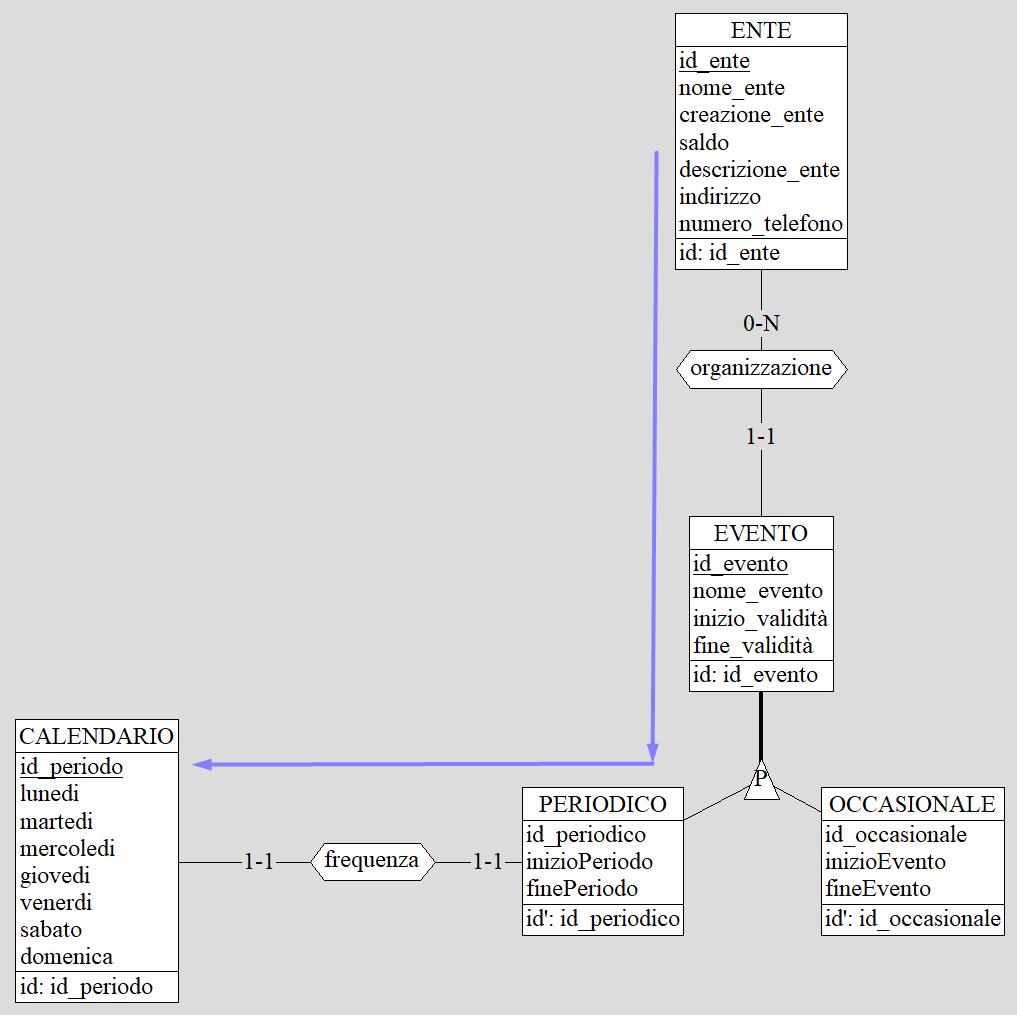
\includegraphics[width=0.95\columnwidth]{c11getEventi.png}
\\
\\
Nella tabella dei servizi disponibili si dovrà mettere anche l'ente fornitore, il prezzo scontato in base all'abbonamento sottoscritto dal cliente.
\subsubsection*{c10. Visualizzare lista eventi}
\begin{longtblr}
[
caption = {Visualizzare lista eventi},
]{
colspec = {|X[3]X[1]X[2]X[4]|},
rowhead = 1,
hlines,
row{even} = {lightgray},
row{1} = {LightCoral},
} 
Concetto & Costrutto & Accessi & Tipo \\
Cliente & E & 1 & L \\
Ente & E & 1 & L \\
Organizza & R & 1 & S \\
Eventi & E & 1 & L\\ 

\SetCell[c=4]{l, white} {
    Totale: 3L + 1S\textrightarrow 7500/giorno\\
    Costo totale: 4 x (7500) = 30000/giorno
    }
\end{longtblr}


% TODO Decidere se lasciare come extra
\subsubsection*{c11. Visualizzazione lista carta di credito}
\begin{longtblr}
[
  caption = {Visualizzazione lista carta di credito},
]{
  colspec = {|X[3]X[1]X[2]X[4]|},
  rowhead = 1,
  hlines,
  row{even} = {lightgray},
  row{1} = {LightCoral},
} 
Concetto & Costrutto & Accessi & Tipo\\

Cliente & E & 1 & L\\ 
Possiede & R & 1 & L \\
Carta di credito & E & 1 & L \\
\SetCell[c=4]{l, white} {
    Totale: 3L \textrightarrow 1500/giorno\\
    Costo totale: 3 x (1500) = 4500/giorno
    }
\end{longtblr}

